根据本研究对流域人水关系的定义以及对稳态转换框架的认识,识别流域系统的稳态转换是分析人水关系变化过程的基础,而分析其驱动力则是明晰变化机制的关键。
本研究对流域人水系统状态的定义植根于社会-生态系统的“稳态”概念,识别稳态需要从“驱动-现象-效应”三要素中多个要素入手,分析复合特征的变化。
换言之,本研究中识别流域稳态时,需要使用特征变化的识别方法对稳态转换的驱动力和现象/效应都进行分析或检验,以确定流域系统内既存在明显的突变现象,又存在相应的稳态转换驱动力。
本章以黄河流域符合上述定义的稳态变化的实证研究为典型案例,总结了人水系统稳态转换研究的分析路径(图\ref{ch2:fig:identifying})。
% ,具体如图所示

最常见的稳态转换识别方法是聚焦于稳态转换过程中所表征出的现象,寻找合适的指标和标准识别系统互馈变量的趋势突变或其他相关解释变量的不连续性,并对直接相关的变量进行检测。
当分析缺乏完整的现象变量数据资料而驱动力明确的稳态转换现象时,可以从驱动因素的阈值效应入手建立指标和标准,也可有效分析稳态转换过程。
结合本章先前对“人水关系”的定义,本研究识别人水关系变化过程及其机制的思路框架是:识别主导流域“自然-社会”二元水循环稳态的关联要素及其稳态变化现象,结合稳态转换的驱动机制(气候变化或人类活动?自上而下或自下而上?),分析利益相关者的与水圈要素过程关联的状态如何变化、因何变化。

\begin{figure}[!htb] % use float package if you want it here
    \centering
    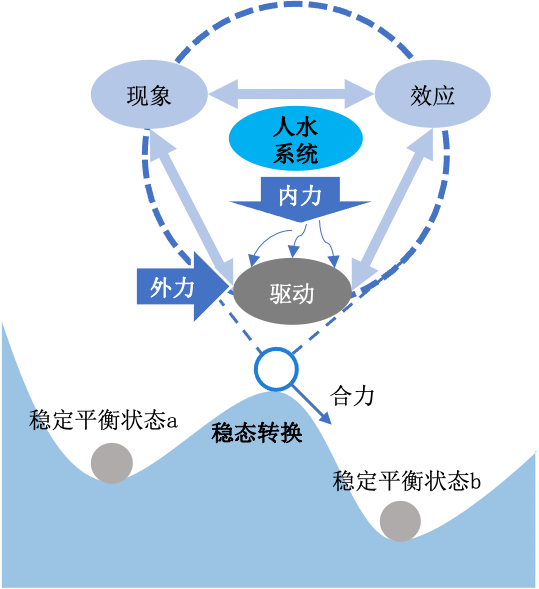
\includegraphics[width=0.5\textwidth]{img/ch2/ch2_framework.png}
    \caption{人水系统稳态转换的分析路径}\label{ch2:fig:identifying}
\end{figure}
